\label{sec:approach}
%
We adopt a neuro-symbolic approach for fast plan recovery by (i) learning a neural model for  $=_\mathcal{S}$ and $\mathcal{K}$ and (ii) searching for a plan $\mathcal{P}$ in a quasi-symbolic space such that the resulting plan takes the robot to a state $S_k$ in minimum number of steps. This subsection first introduces a representation for the robot's environment in the form of a scene-graph. Following which the learned transition model and the discriminator function are introduced. Finally, the details of the learning-aided recovery planning are presented. 

\subsection{Scene-Graph Representation ($\mathcal{Z}, \phi$)}
\label{subsec:sgs}
The visual information ($S \in \mathcal{S}$) fed into the neuro-symbolic planner \cite{Kalithasan2022LearningNP}, $\mathcal{M}$, consists of an RGB-D image and bounding boxes of all the objects in the inital table-top state. The model $\mathcal{M}$ uses a \textit{visual extractor} (VE) module to extract feature-vectors for every object in the state. We assume that there are no completely occluded objects, which otherwise will not be perceived by $\mathcal{M}$. Therefore, for each object, we use the VE module to get its feature-vector and bounding box with depth. We concatenate these two and pass it through an MLP-based \textit{encoder} ($E_N$) to get the final object representation, referred to as \textit{node-embedding} in subsequent discussions. The network $E_N$ is trained jointly with the Scene-Graph Predictor (see subsection~\ref{subsec:sgp}).

Next, for each pair of object, we form the \textit{edge-embedding} by simply concatenating the corresponding pair of \textit{node-embeddings}. The order of concatenation matters as the relations in real-world (like top, left and right) are not symmetric, and hence, there are two edges for every pair of objects, giving a total of $n \times (n - 1)$ edges, where $n$ is the number of objects in the scene. The \textit{node-embeddings} along with the \textit{edge-embeddings} form the scene-graph $Z$, for the given state $S \in \mathcal{S}$. The set of all such $Z$ forms the Scene-Graph Space $\mathcal{Z}$.
%
We denote the transformation of a state $S \in \mathcal{S}$ to its scene-graph $Z \in \mathcal{Z}$ by the function, $\phi: \mathcal{S} \rightarrow \mathcal{Z}$. 
%As mentioned previously, some aspects of this transformation are pre-trained and frozen (using $\mathcal{M}$), while other are trained jointly with the Scene-Graph Predictor (i.e., $E_N$).

\subsection{Learning the Scene-Graph Predictor ($\mathcal{T}$)}
\label{subsec:sgp}
In this subsection, we plan to model the effect of executing a symbolic action $\pi \in \mathcal{A}$ on a scene-graph $Z \in \mathcal{Z}$. Essentially, we want to learn a function, $\mathcal{T}: \mathcal{Z} \times \mathcal{A} \rightarrow \mathcal{Z}$, such that for any $S \in \mathcal{S}$, $\mathcal{K}(S, \pi) \equiv \mathcal{T}(\phi(S), \pi)$. Here, $\mathcal{T}$ is the scene-graph predictor that takes as input a scene-graph and a symbolic action, and outputs the \textit{intended} scene-graph. By \textit{intended}, we mean the scene-graph which otherwise $\mathcal{M}$ will extract from the table-top state $S$ after executing the symbolic action. 

We propose a neuro-symbolic architecture for $\mathcal{T}$ and train it on examples consisting of initial ($S_I$) and final ($S_F$) table-top states and a symbolic action $\pi$, such that $\mathcal{K}(S_I, \pi) =_\mathcal{S} S_F$. The plan ($(\pi)$) is provided to us by the model $\mathcal{M}$. Figures ~\ref{fig:scene-graph-predictor} and ~\ref{fig:sgp} give an overview of the model architecture, and its training paradigm. Both $\mathcal{T}$ and $\phi$ are trained jointly and via backpropagation of corresponding losses.

\begin{figure}
    \centering
    \begin{subfigure}{0.45\textwidth}
        \centering
        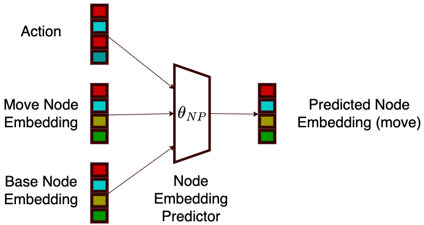
\includegraphics[width=\textwidth]{assets/node-predictor1.png}
    \end{subfigure}
    \begin{subfigure}{0.45\textwidth}
        \centering
        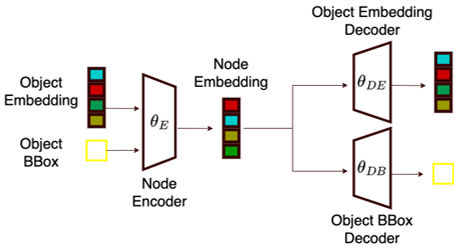
\includegraphics[width=\textwidth]{assets/node-predictor-2.png}
    \end{subfigure}
    \caption{\textbf{Scene-Graph Predictor.} It inputs a scene graph and action and predicts a new embedding for the moved object node. The node embeddings are obtained by encoding object embeddings and their bounding boxes}
    \label{fig:scene-graph-predictor}
\end{figure}

\begin{figure}
    \begin{subfigure}{1.0\hsize}
         \centering    
         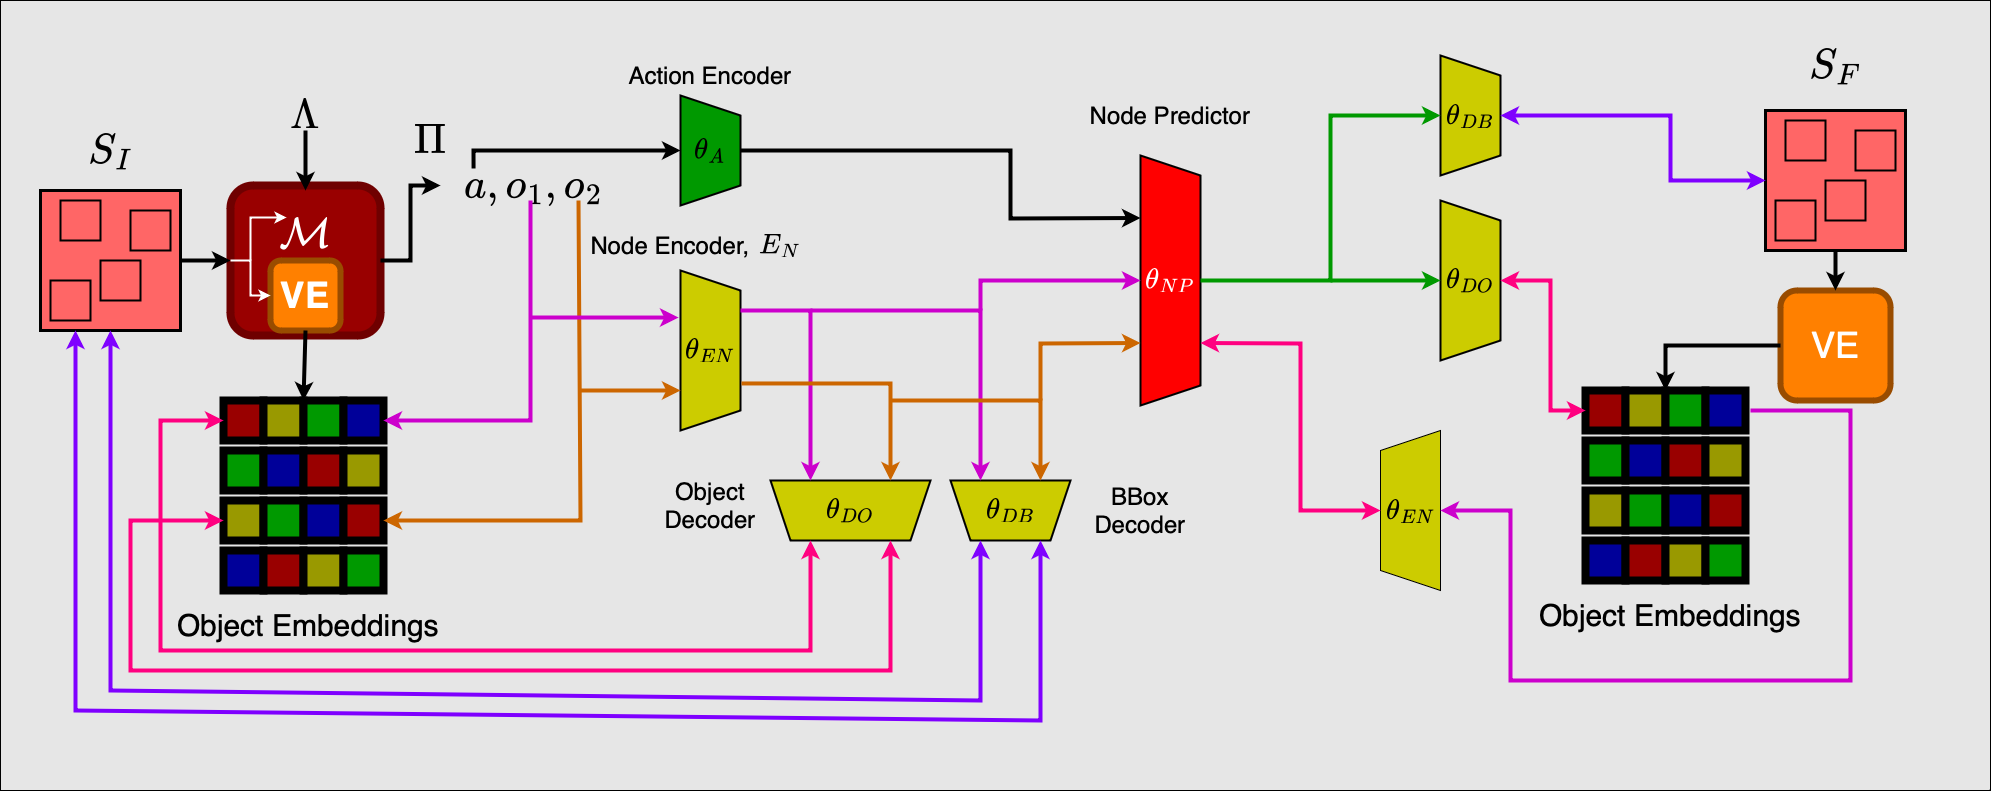
\includegraphics[width=\textwidth]{figures/sgp-7.png}
    \end{subfigure}
    \caption{\textbf{Training the scene-graph predictor. }Double-headed arrows represent loss calculation. Purple: MSE, Red-pink: MSE + IoU (for bounding box)). 
    }
    % \vspace{-0.15in}
    \label{fig:sgp}
\end{figure}

Once we have $\mathcal{T}$ trained, given initial state $S \in \mathcal{S}$ and $T$-length plan $\Pi \in \mathcal{P}$, we can evaluate intermediate scene-graphs for each $t \leq T$ as $Z_t = \mathcal{T}(Z_{t-1}, \pi_t)$, where $Z_0 = \phi(S)$. This is useful as it provides us the ability to \textit{imagine} and get an idea of the actual table-top setting including object relations via $Z_i's$ without actually executing the plan on the robot. This makes the \textit{imagined} scene-graphs robust to physical errors and useful for comparison with actual states during robotic execution. Figure~\ref{fig:rollout} shows the execution of a plan on a table-top setting and compares it with images reconstructed using the corresponding predicted scene-graphs.

\subsection{Learning the Scene-Graph Discriminator ($=_\mathcal{Z}$)}
\label{subsec:sgd}
The similarity (or dissimilarity) between scene-graphs is estimated using a discriminator model as a function, $=_\mathcal{Z}: \mathcal{Z} \times \mathcal{Z} \rightarrow \{0, 1\}$, such that for any $S_1, S_2 \in \mathcal{S}$, $S_1 =_\mathcal{S} S_2 \iff \phi(S_1) =_\mathcal{Z} \phi(S_2)$. Here, $=_\mathcal{Z}$ is the scene-graph discriminator that takes as input two scene-graphs and outputs either $0$ (unequal) or $1$ (equal). Since, the edges in scene-graph are a function of the nodes, we can discriminate between two graphs by discriminating between the two \textit{node} sequences. So, we break learning of $=_\mathcal{Z}$ into learning of $=_\mathcal{N}$, which is the discriminator over the node-embedding space $\mathcal{N}$ using the following first-order logic equation:
\begin{equation}\label{eqn:esg}
    Z_1 =_\mathcal{Z} Z_2 \iff \forall \, i \leq n : (o_{Z_1})_i =_\mathcal{N} (o_{Z_2})_i
\end{equation}
Here, $o_{Z_1}$ and $o_{Z_2}$ are the corresponding node-embeddings for $Z_1$ and $Z_2$ respectively. We used an MLP to learn the $=_\mathcal{N}$ function. See figure~\ref{fig:disc-arch} for the discriminator architecture. The discriminator is trained once the training of the scene-graph predictor is complete. The data set used for training is the same as in subsection~\ref{subsec:sgp}. For a given example triplet $(S_I, \Pi, S_F)$, where $\Pi = ((a_1, o_{11}, o_{21}))$, the scene-graph is extracted using $\phi$ to get $Z_I$ and $Z_F$. Assuming there are $n$ objects in the scene, a total of $n^2$-pairs of node-embeddings are formed. We treat pairs of the form $((o_{Z_I})_i, (o_{Z_F})_j)$ as negative examples (i.e., label $= 0$), for all $i \neq j$. When $i = j$, we treat $((o_{Z_I})_{o_{11}}, (o_{Z_F})_{o_{11}})$ as negative example (label $= 0$) and remaining as positive examples (label $= 1$). Hence, the learning is self-supervised and the network is trained via back-propagation of cross-entropy loss.

\begin{figure}
    \centering
    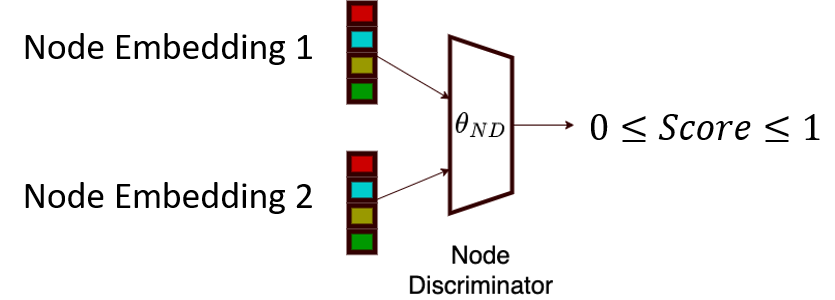
\includegraphics[width=0.6\textwidth]{assets/discriminator.png}
    \caption{\textbf{Scene-Graph Discriminator}. It takes 2 scene graphs as input and disriminates between their node sequences}
    \label{fig:disc-arch}
\end{figure}

Once we have $=_\mathcal{N}$ trained, we can evaluate $=_\mathcal{Z}$ for any two scene-graphs using Equation~\ref{eqn:esg}. This allows us to detect errors in robotic execution by comparing the scene-graphs predicted recursively using $\mathcal{T}$ and extracted from the actual table-top state (using $\phi$) at run-time. 
%
The learned discriminator network is then used to estimate which objects are potentially involved in the error by computing a  \emph{discrepancy} function $\mathcal{D}: \mathcal{Z} \times \mathcal{Z} \rightarrow \mathbb{Z}_{\geq 0}$\textit{.} 
%
This function can be used to estimate a heuristic distance between two world states (represented as scene graphs ) as $Z_1$ and $Z_2$ as   
%
\begin{equation}
    \mathcal{D}(Z_1, Z_2) =  n - \sum_{i = 1}^{n} \mathbbm{1}_{\{(o_{Z_1})_i =_\mathcal{N} (o_{Z_2})_i\}}.
\end{equation}
%
Here, $o_{Z_1}$ and $o_{Z_2}$ are the corresponding node-embeddings for $Z_1$ and $Z_2$ respectively. 
%
This function serves as heuristic to guide our search in the planning space $\mathcal{P}$ which is described next.

\subsection{Neuro-symbolic Search for Recovery Plan $\mathcal{P}$}
\label{subsec:plan}
Our recovery strategy searches for a plan from the current state to a sub-goal along the original plan, while respecting the sub-goals already obtained. Using $\mathcal{T}$ and $=_\mathcal{Z}$, the plan is formulated using a forward search in the quasi-symbolic space ($\mathcal{Z}$) where the robot reasons over sequence of actions which in turn are realised as neural modules grounded over the robot’s state space. The discrepancy function $\mathcal{D}$ is used as the state's heuristic value. The search is made efficient in three ways. 
\begin{enumerate}
    \item We perform data-driven learning of pre-conditions for actions in the form of neural functions on the state. These functions capture when an action can be applied and chained in succession enabling pruning of irrelevant branches.
    \item Manipulation tasks such as stacking or assembly often make space of free space to stack while positioning items relative to another (e.g., on top). Instead of explicitly reasoning over a multitude of metric poses, we lean a transformer-neural function that predicts collision-free poses for a given world state. The learned neural model off-loads the search over metric poses from symbolic planner thereby making the combined neuro-symbolic search efficient.
    \item We make use of the discrepancy function to detect exactly which nodes/objects are correctly positioned, and also the symbolic plan executed up till now to determine relations between objects in the scene (like left, right, on top etc.) (Figure ~\ref{fig:pruning}). Knowing which objects are correctly positioned and the relation of incorrectly placed objects with correctly placed ones helps considerably in pruning down the action space and making the search faster.
\end{enumerate}  

\begin{figure}
    \centering
    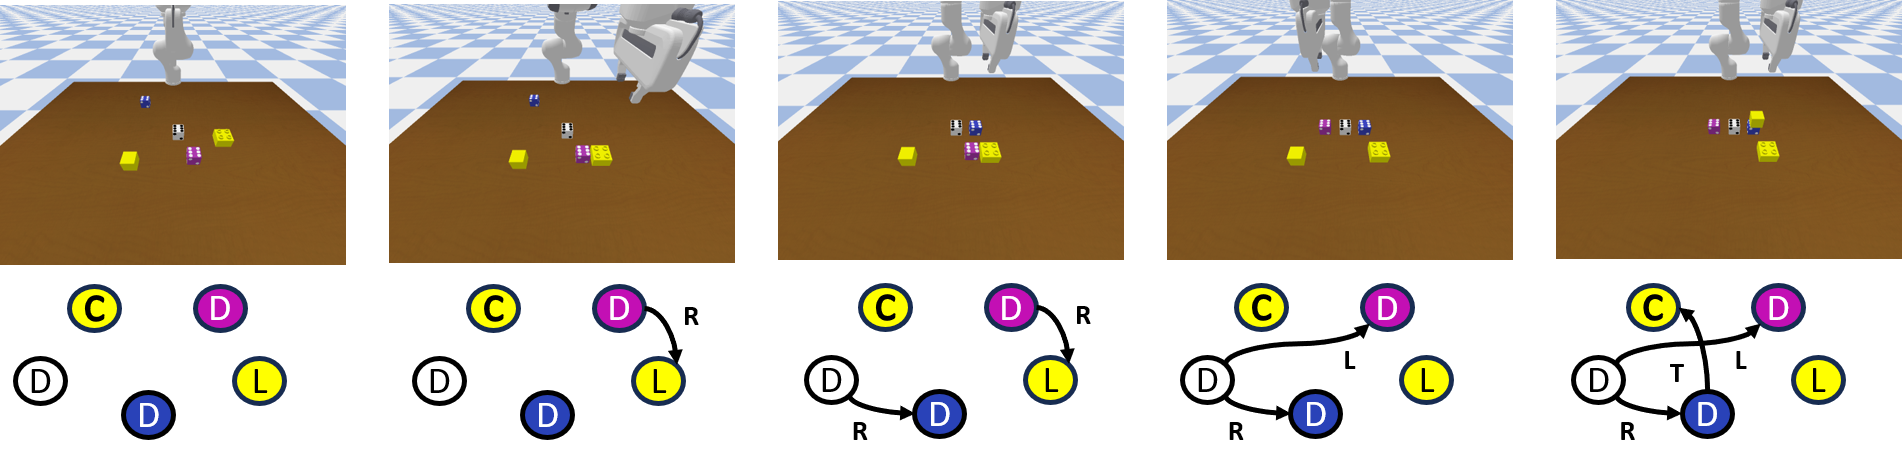
\includegraphics[width=\textwidth]{assets/pruning.png}
    \caption{Determining relations between objects based on the plan to help prune search}
    \label{fig:pruning}
\end{figure}

We discuss approaches for learning action pre-conditions and predicting collision-free spaces in the next sections. The details of our pruned forward search follow. 
%
Given an initial scene $S \in \mathcal{S}$ and a symbolic plan $\Pi = (\pi_1, \pi_2, .., \pi_T) \in \mathcal{P}$, the \textit{intended} intermediate states are $S_1, S_2, ..,$ and $S_T$ (see subsection~\ref{sec:problem2}). Using $\mathcal{T}$, $\phi$ and $S$, we can determine the corresponding \textit{intended} scene-graphs, as $Z_t = \mathcal{T}(Z_{t-1}, \pi_t)$, where $Z_0 = \phi(S)$. 

Now, assume that the first \textit{disturbance} occurred while executing $\pi_t$ on $S_{t - 1}$ resulting in a state $S_t'$, such that $S_t' \neq_\mathcal{S} S_t$. We check the equality using the learnt discriminator function $=_\mathcal{Z}$. Now our aim is to generate a plan $\Pi_{E(t)}$ such that $\mathcal{E}(S_t', \Pi_{E(t)}) =_\mathcal{S} S_k$ for some $k \leq T$. We first solve the problem of planning to an intermediate state in equivalent scene-graph space using forward-search (A$^*$) with the help of $\mathcal{T}$, $=_\mathcal{Z}$ and $\mathcal{D}$. Later, we will solve the problem of detecting the optimal intermediate state $S_k$ to plan to for \textit{fast} recovery. For the A$^*$-search, the starting state is $Z_I := \phi(S_t')$, goal-state is $Z_k$, goal-check function is $=_\mathcal{Z}$ and the heuristic function is $\mathcal{D}$. The space of actions is originally the entire $\mathcal{A}$, i.e., all symbolic action triplets of the form (\texttt{top}/\texttt{left}/\texttt{right}, $o_1$, $o_2$). However, to make the search efficient, we prune the set of actions that can be taken at any intermediate scene-graph ($Z$) using node \textit{discriminator} network, $=_\mathcal{N}$. Let the number of objects in $Z$ and $Z_k$ be $n$. Then for each $i \leq n$, we mark node as \texttt{correct} if $(o_{Z})_i =_\mathcal{Z} (o_{Z_k})_i$, and \texttt{incorrect} otherwise. Now, we use the following heuristics to prune the action space:
% \vspace{-0.7em}
\begin{itemize}
    % \setlength\itemsep{-0.2em}
    \item For \texttt{incorrect} nodes (say id $i$), we lookup its symbolic relation with other nodes in the goal scene-graph. This can be done either by looking at the sequence of symbolic actions $(\pi_1, \pi_2, .., \pi_k)$ leading to $Z_k$ (from $Z_0$), or by explicitly evaluating the symbolic relation using neural operator (left, right, on top etc.) on the edge embeddings in the scene-graph, $Z_k$. If it is symbolically related (say relation $a$) with some other node in the scene-graph (say id $j$), we prune all actions except $(a, i, j)$. Here $a$ is \texttt{top}, \texttt{left} or \texttt{right}. Otherwise, we prune all symbolic actions and add a new action (\texttt{mov}, $i$), which simply moves the node $i$ to its actual position in $S_k$, which is extracted from $Z_k$ via neural object bounding box decoder (see Figure~\ref{fig:sgp}).
    \item For \texttt{correct} nodes, we prune all symbolic actions.
    \item For each node (say id $i$), we add a new action (\texttt{free}, $i$), which simply moves the node $i$ to a position which is collision-free in both current and goal scene-graphs/states. Instead of explicitly reasoning over a multitude of metric positions, we learn a transformer-based neural network that predicts the required collision-free position. The learnt neural model off-loads the search over metric positions from the symbolic planner making the combined neuro-symbolic search efficient.
\end{itemize}
The action space is further pruned by using preconditions learnt for different symbolic actions. The precondition model is a neural network learnt in a supervised manner from both positive and negative examples of initial states, and uses object-relations extracted from scene-graph edges as input. For a given symbolic action, the model outputs \textit{true} if the action can be performed and \textit{false} otherwise.

For the basic version of our approach, we set $Z_k = S_t$, that is we recover to the next intermediate state when a discrepancy was detected while executing $\pi_t$ on $S_{t-1}$. In the next section, we motivate and explore an \textit{anytime} version of our approach.

\subsection{Anytime recovery}

While recovering to the next intermediate state $S_t$ works well in most cases, there may be situations where recovering to another intermediate state $S_k$ would lead to faster recovery. See figure ~\ref{fig:anytime} for a motivational example. The 3-step input instruction, "Put the green cube on top of the yellow cube and put the red cube on top of the green cube and put the green lego on top of the red cube", corresponds to building a tower of 4 blocks. Let $S_1$ be the initial state, and $S_{2-4}$ correspond to the states with 2-4 blocks in the tower respectively. 
In the first case, after the $S_4$ is reached, an adversarial agent resets the state to $S_2$ by putting top two objects of the tower at their original locations. Here, our earlier approach would recover to $S_4$. However, choosing $Z_k=S_2$ leads to faster recovery as the original plan from $S_2$ to $S_4$ can be reused. 
In the second case, after state $S_2$, a cooperative agent helps the robot by executing the next action and reaching state $S_3$. Here, our earlier approach would recover to $S_2$ and unnecessarily un-stack the block again, leading to a total plan length of 3 to reach the goal. Choosing $Z_k=S_3$ leads to faster recovery as the goal is reached in just a single step.

We thus extend the discrepancy-aware planning framework to find the nearest state on the original trajectory, that is find the optimal $S_k$ to recover.
Since the trajectory may be long, determining $k$ itself may take long time. So, we bound this overhead by a budget $K$, denoting the number of states to which the algorithm is allowed to plan simultaneously.

The anytime recovery algorithm is then as follows:
\begin{enumerate}
    \item Use Scene-Graph Predictor to find all intended intermediate states $S_1, S_2, ... S_T$
    \item Sort the states based on their discrepancy value with the current state $S_t$, and choose the top-K states with least discrepancy values.
    \item Plan simultaneously to these top-K states, using modified A* - search: (i) An admissible heuristic is formed by taking the minimum of all discrepancy values. (ii) Discrepancy-Aware Pruning is done for multiple goal-states (iii) The plan to the first encountered goal-state is returned
\end{enumerate}

\begin{figure}
    \centering
    \begin{subfigure}{\textwidth}
        \centering
        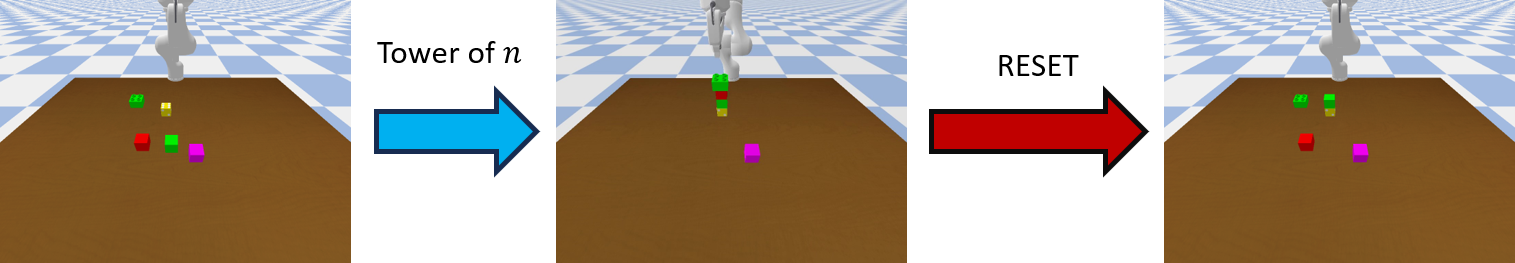
\includegraphics[width=\textwidth]{assets/anytime-1.png}
        \caption{An \textbf{Adversarial} agent resets the state to some intermediate state.}
    \end{subfigure}

    \vspace{0.5cm}

    \begin{subfigure}{\textwidth}
        \centering
        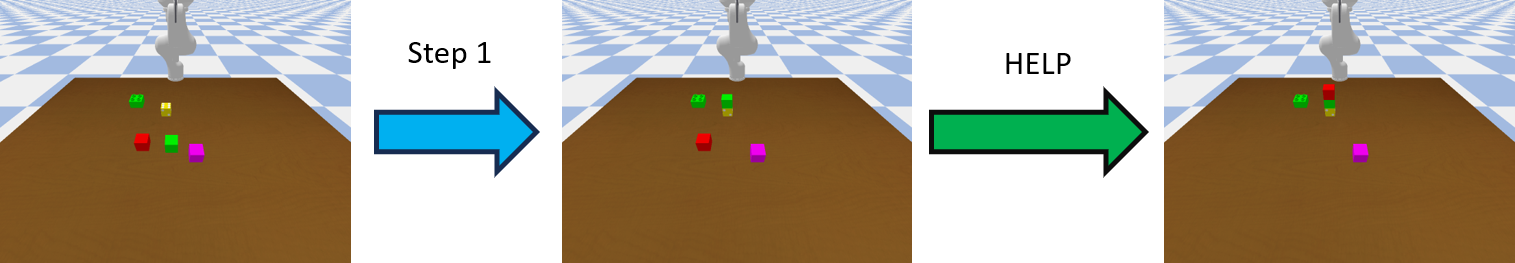
\includegraphics[width=\textwidth]{assets/anytime-2.png}
        \caption{A \textbf{Cooperative} agent helps the robot by executing the next intended action
}
    \end{subfigure}

    \caption{Motivation for anytime recovery}
    \label{fig:anytime}
\end{figure}


% For anytime variant of our algorithm, we simply sort all sub-goals based on the value of discrepancy function and select \textit{top-K} closest sub-goals (least discrepancy). We find plans to reach either of the selected sub-goals and return the shortest one.


\subsection{Free-Space Transformer}
To generate a collision-free position while executing "free" action on current state, we extract the bounding boxes of the objects in the current and goal scene-graphs using object bounding box decoder (in scene-graph predictor) and concatenate them together to form a single 2D tensor consisting of all the bounding boxes that the we need to avoid placing the object at. This 2D tensor along with the ID of the object to be manipulated is then passed through a transformer architecture ~\cite{Vaswani2017AttentionIA} that outputs the resulting position (bounding box) where the object should be placed to avoid collision. See Figure~\ref{fig:free-arch} for the architecture. The network is trained on a dataset consisting of a single scene with bounding boxes for all the objects provided. We use two losses to train the network: First is an MSE Loss between the predicted bounding box and the original bounding box of the manipulated object. This loss ensures that the predicted position is in vicinity of the original position of the object and the predicted position actually represents a valid object bounding box. Second is an IoU loss that is taken between the predicted bounding box and the bounding boxes of all the objects in the scene. This loss ensures that the position is collision-free.

\begin{figure}
    \centering
    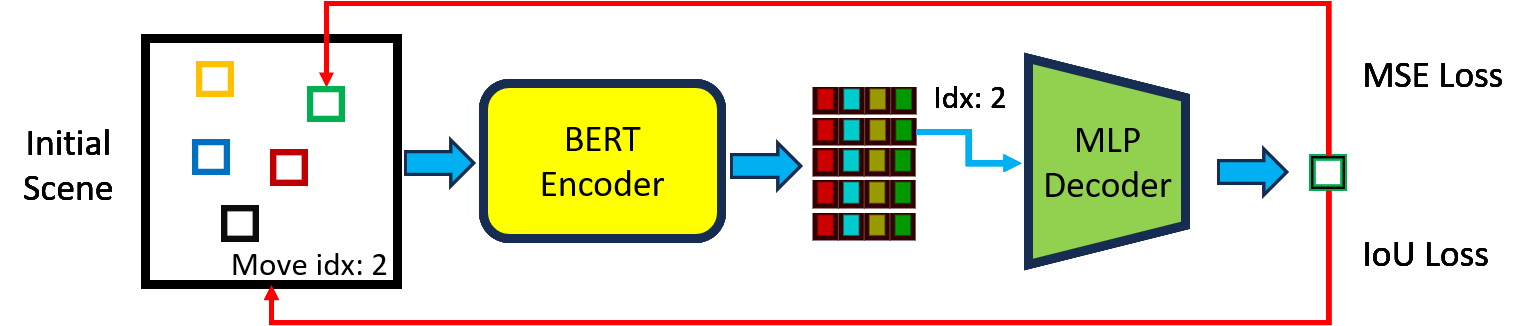
\includegraphics[width=\textwidth]{part-2/free-arch.png}
    \caption{Architecture of free-space module}
    \label{fig:free-arch}
\end{figure}

\begin{figure}
    \begin{subfigure}{0.5\hsize}
         \centering    
         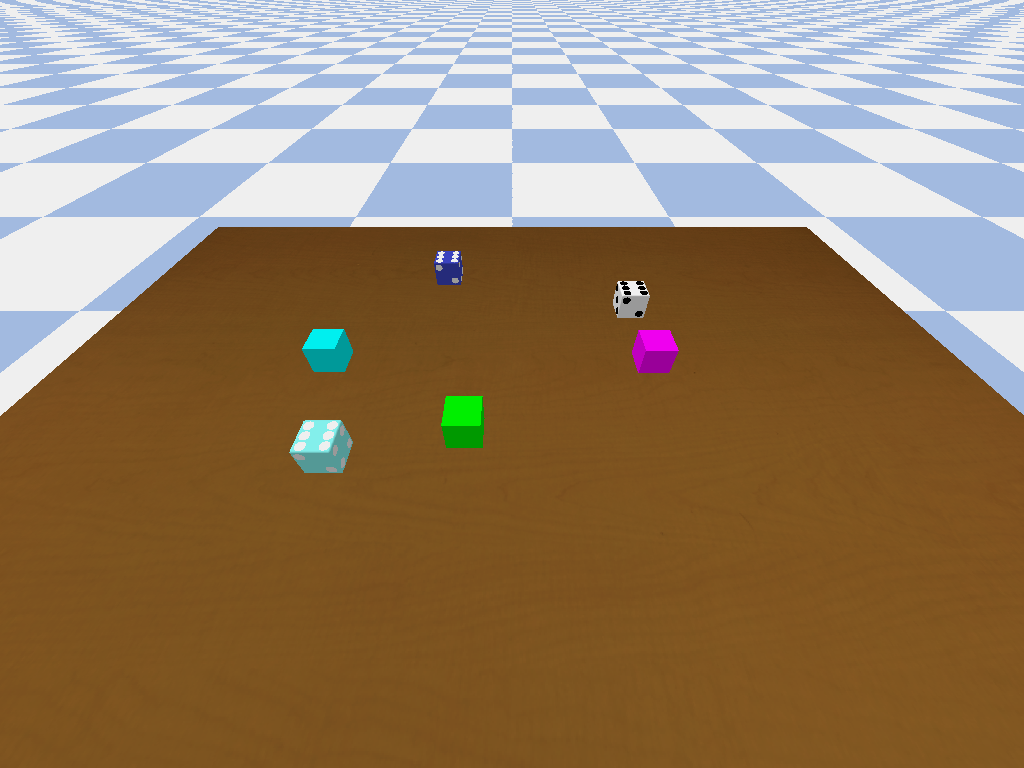
\includegraphics[scale=0.19]{figures/rze_i.png}
         \caption{The initial scene where the task is to move the \textit{cyan lego} to a collision free position.}
    \end{subfigure}
    \begin{subfigure}{0.5\hsize}
         \centering    
         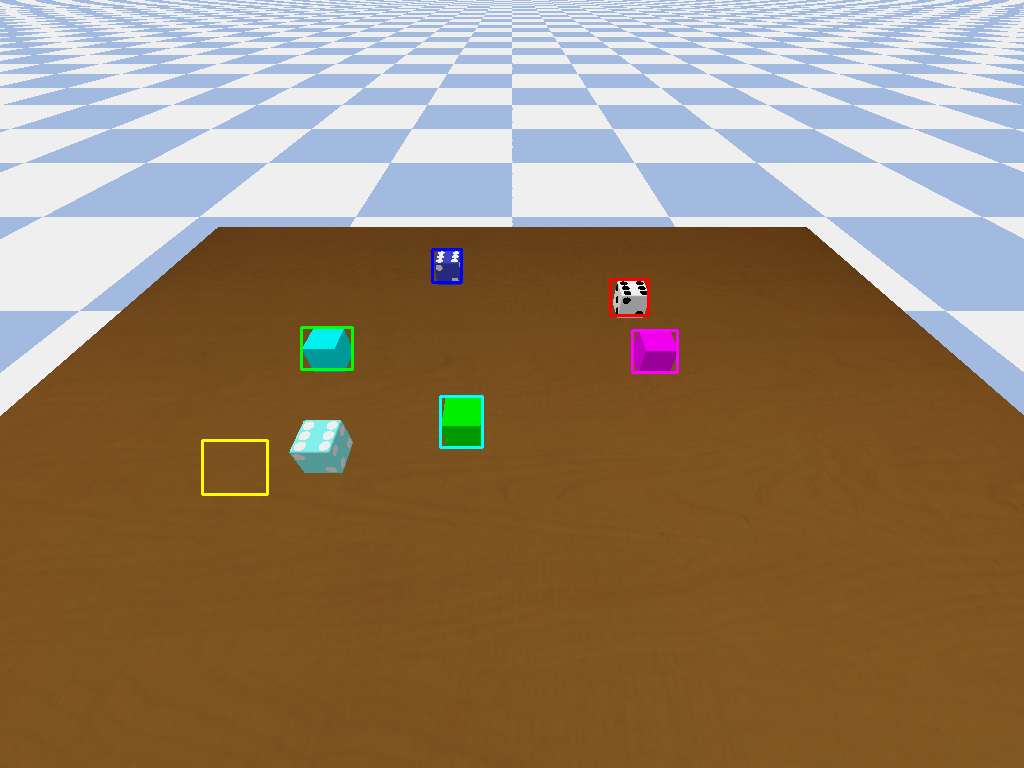
\includegraphics[scale=0.19]{figures/rze_pre.png}
         \caption{The predicted collision free position for the \textit{cyan lego}. (yellow bounding box)}
    \end{subfigure}
    \caption{
            Output of \textit{free}-space module. 
    }
    % \vspace{-0.15in}
    \label{fig:free-space}
\end{figure}

\subsection{Precondition Network}
To train the precondition network, we generate dataset of initial and final states and manipulation program (single action). The dataset also contains labels denoting whether the action can be executed or not (Positive/Negative examples). We extract \texttt{onTop}, \texttt{onLeft} and \texttt{onRight} relations for \textit{subject} and \textit{object} nodes for manipulation with all the other objects present in the scene. This is done by applying MLP-based networks on the edge embeddings of the scene-graph. These MLPs are trained via self-supervision on the original corpus consisting of initial and final states and single symbolic action. We pass the value of these predicates to an MLP (precondition-network) and supervise it with labels (Positive/Negative) present in the dataset. The network is trained via backpropagation of the cross-entropy loss. See Figure~\ref{fig:precond} for the network architecture.

\begin{figure}
    \centering
    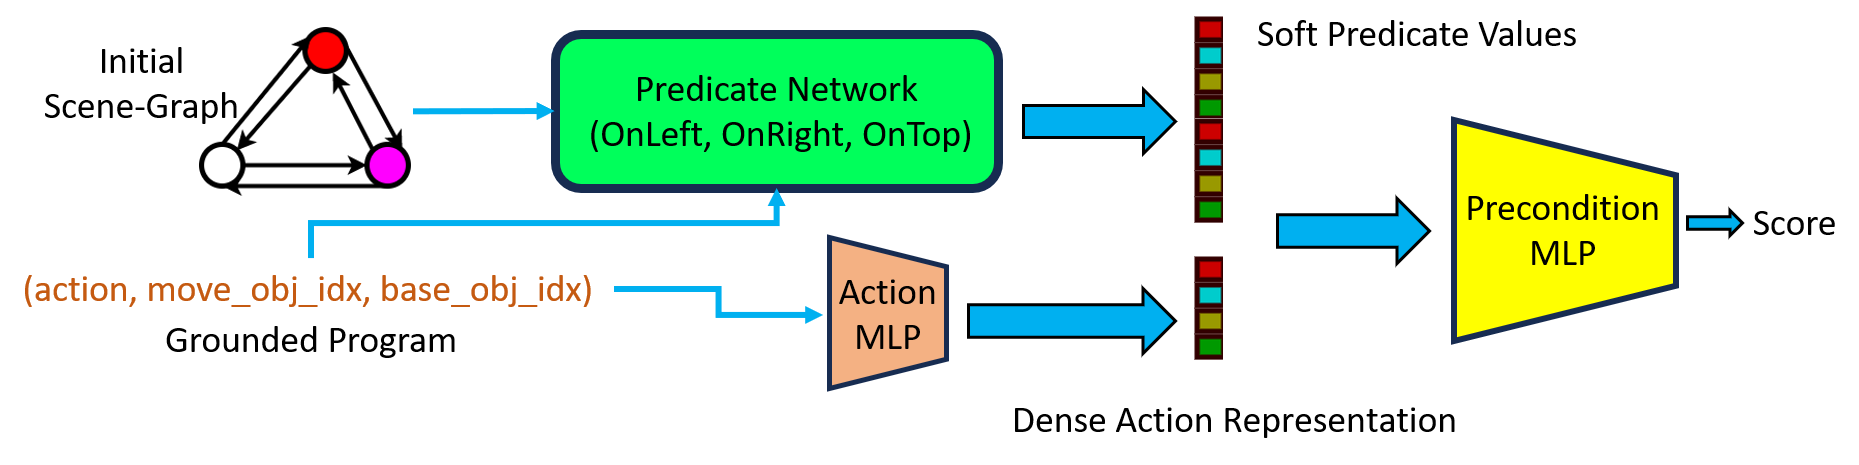
\includegraphics[width=\textwidth]{assets/precond.png}
    \caption{Precondition Network architecture}
    \label{fig:precond}
\end{figure}